\chapter{Schaltplan}
\label{appendix:schaltplan}
Auf der Folgeseite ist der Schaltplan der esten Iteration aufgeführt. Er wird in \enquote{fritzing} erstellt und beinhaltet alle elektrische Komponenten, welche im Boot verbaut sind.

Darauffolgend ist die Schematik der Platine aufgeführt. Diese ist in KiCad, einem Open source ECAD Program erstellt.

\begin{figure}[H]
    \centering
    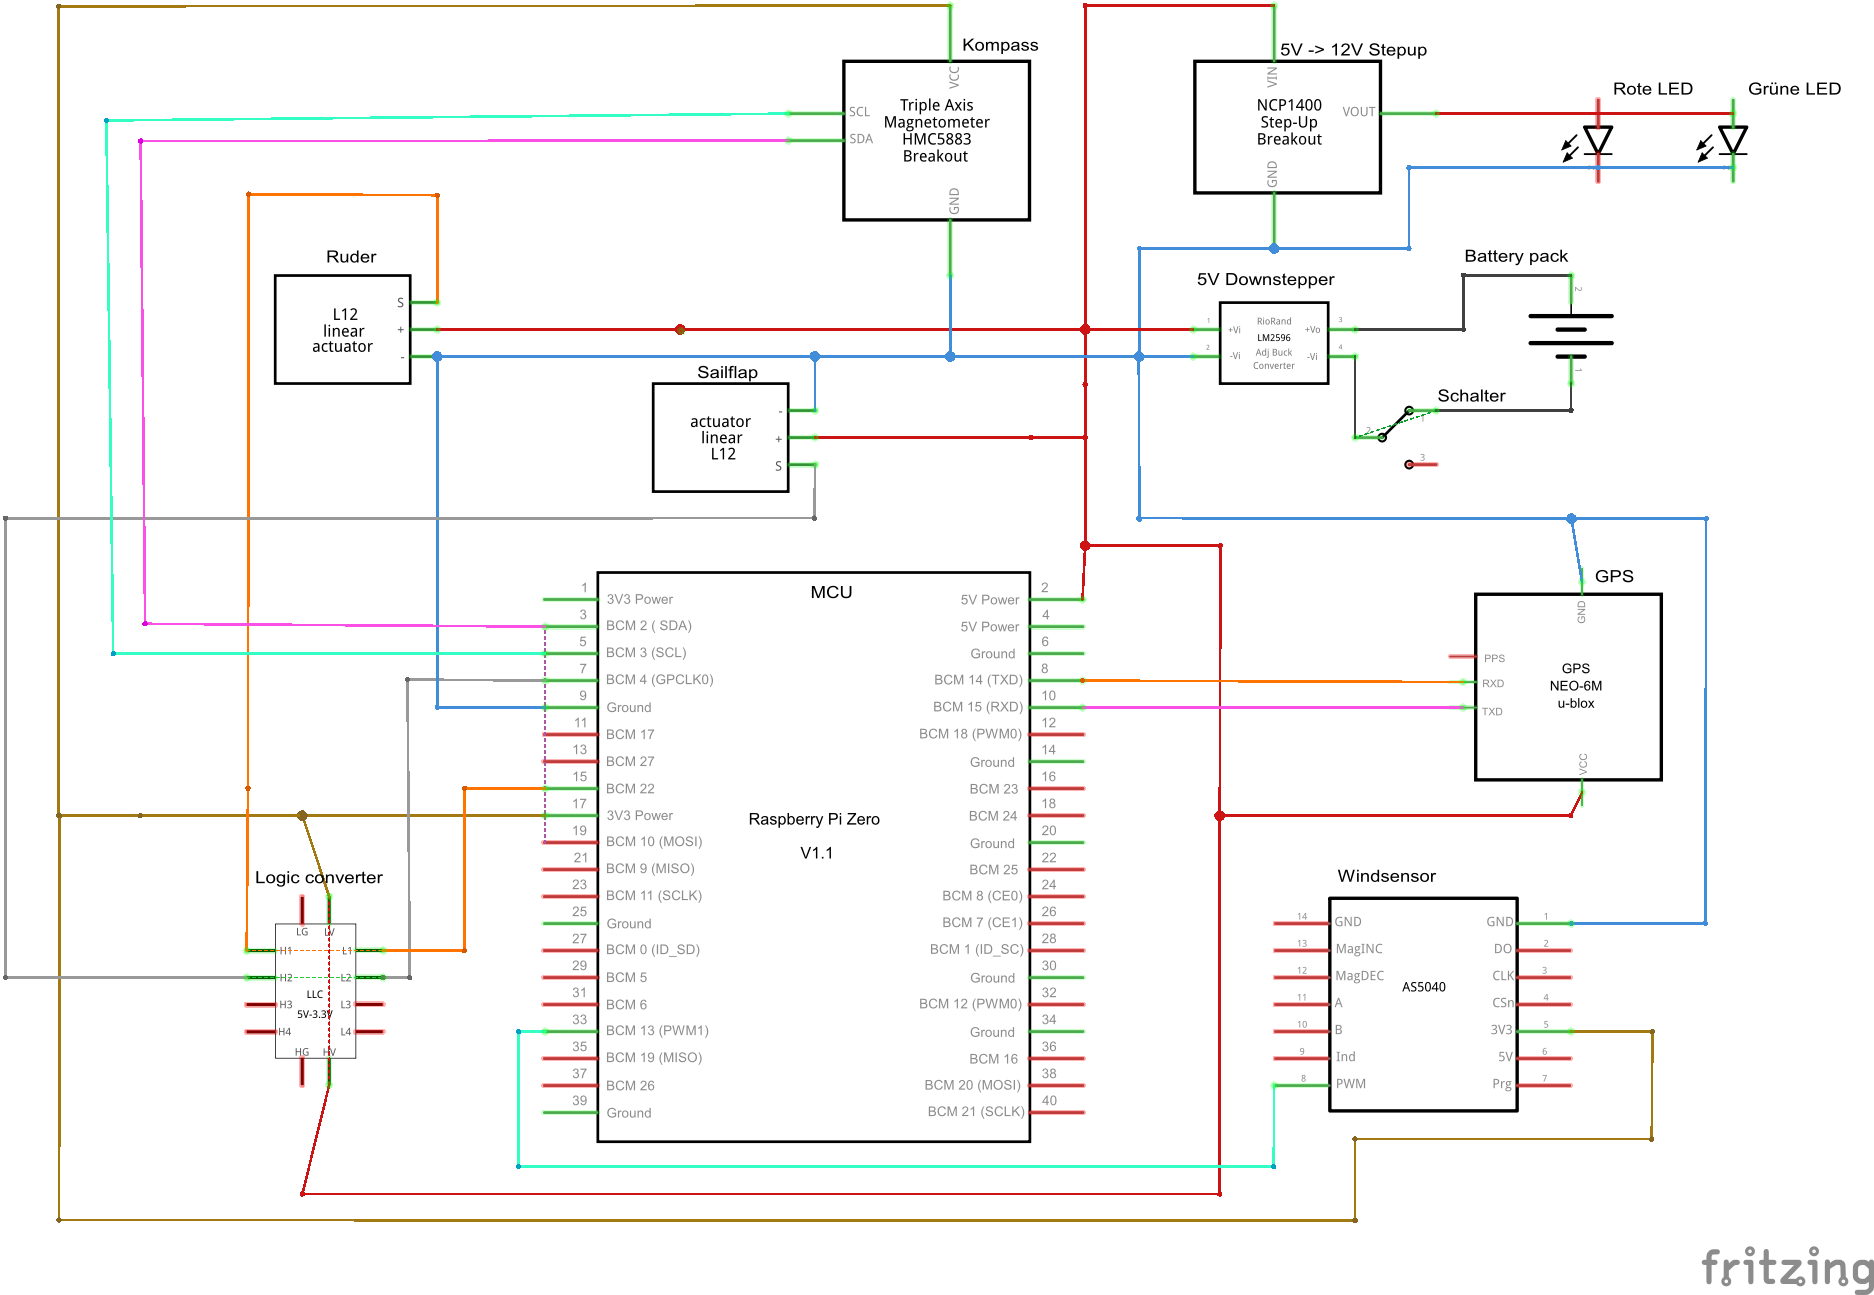
\includegraphics[angle=90,width=\textwidth,height=\textheight,keepaspectratio]{assets/Boat Electronics3_Schaltplanfinal.png}
    \caption{Schaltplan Bordelektronik}
\end{figure}
